
  \section[ML Bank]{Standard ML Results}
  \label{app:standard_bank}

  Appendix \ref{app:standard_bank} contains the standard ML results for the 
  bank telemarketing dataset and is shown in table \ref{table:standard_bank}.

  \begin{table}
    \centering
    \scalebox{1.0}{
    \begin{tabular}{|l||l|l|}
      \hline
      \textbf{ML Method} & \textbf{Training Accuracy} & \textbf{Validation
      Accuracy} \\
      \hline\hline
      Support Vector Machine & 91.54\% & 88.61\% \\\hline
      ANN & 90.25\% & 88.33\% \\\hline
      Random Forest & 100\% & 88.75\% \\
      \hline
    \end{tabular}}
    \caption{Standard ML Results Bank Telemarketing Dataset}
    \label{table:standard_bank}
  \end{table}

  \section[Deterministic Graph]{Deterministic Graph Results}
  \label{app:det_graphs}

  Appendix \ref{app:det_graphs} contains the results for the deterministically 
  generated \acs{mag} presented in section \ref{section:stoch_det}. Figure 
  \ref{fig:det_plots} and table \ref{table:det_plots} show the GraphSage 
  results using max-pooling.

  \begin{figure}
		\centering
		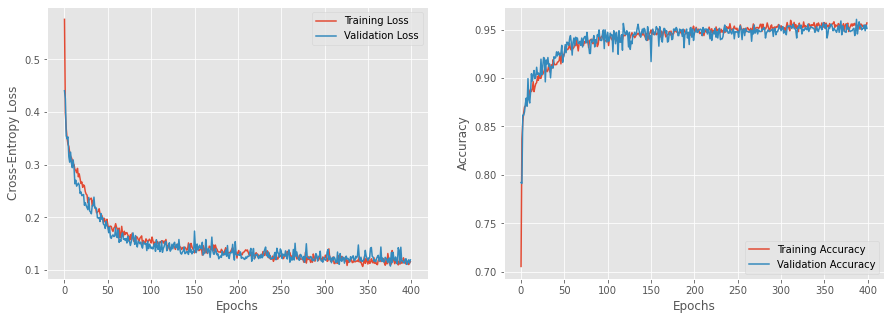
\includegraphics[width=0.9\textwidth]{GraphSage_det_plots.png}
		\caption{Max-Pooling Loss- and Accuracy Plots Deterministic MAG}
        \label{fig:det_plots}
  \end{figure}

  \begin{table}
    \centering
    \begin{tabular}{|l|c|c|}
      \hline
      \diagbox{\textbf{Label}}{\textbf{Predicted}} & \textbf{Neutral or
      Dissatisfied} & \textbf{Satisfied}\\
      \hline
      \textbf{Neutral or Dissatisfied} & 3'167  & 163 \\\hline 
      \textbf{Satisfied} & 191 & 2'479 \\\hline\hline
      \textbf{Accuracy} & 94.10\% & \\
      \hline
    \end{tabular}
    \caption{Test Confusion Matrix Deterministic MAG}
    \label{table:det_plots}
  \end{table}

  \section[Pairplot]{Pairplot of US Airline Passenger Dataset}
  \label{App:pairplot}

  Appendix \ref{App:pairplot} contains the pairplot of the feature data of the 
  US airline passenger dataset referenced in section 
  \ref{section:informativeness} is depicted in figure \ref{fig:pairplot_feature}.

  \begin{figure}
		\centering
		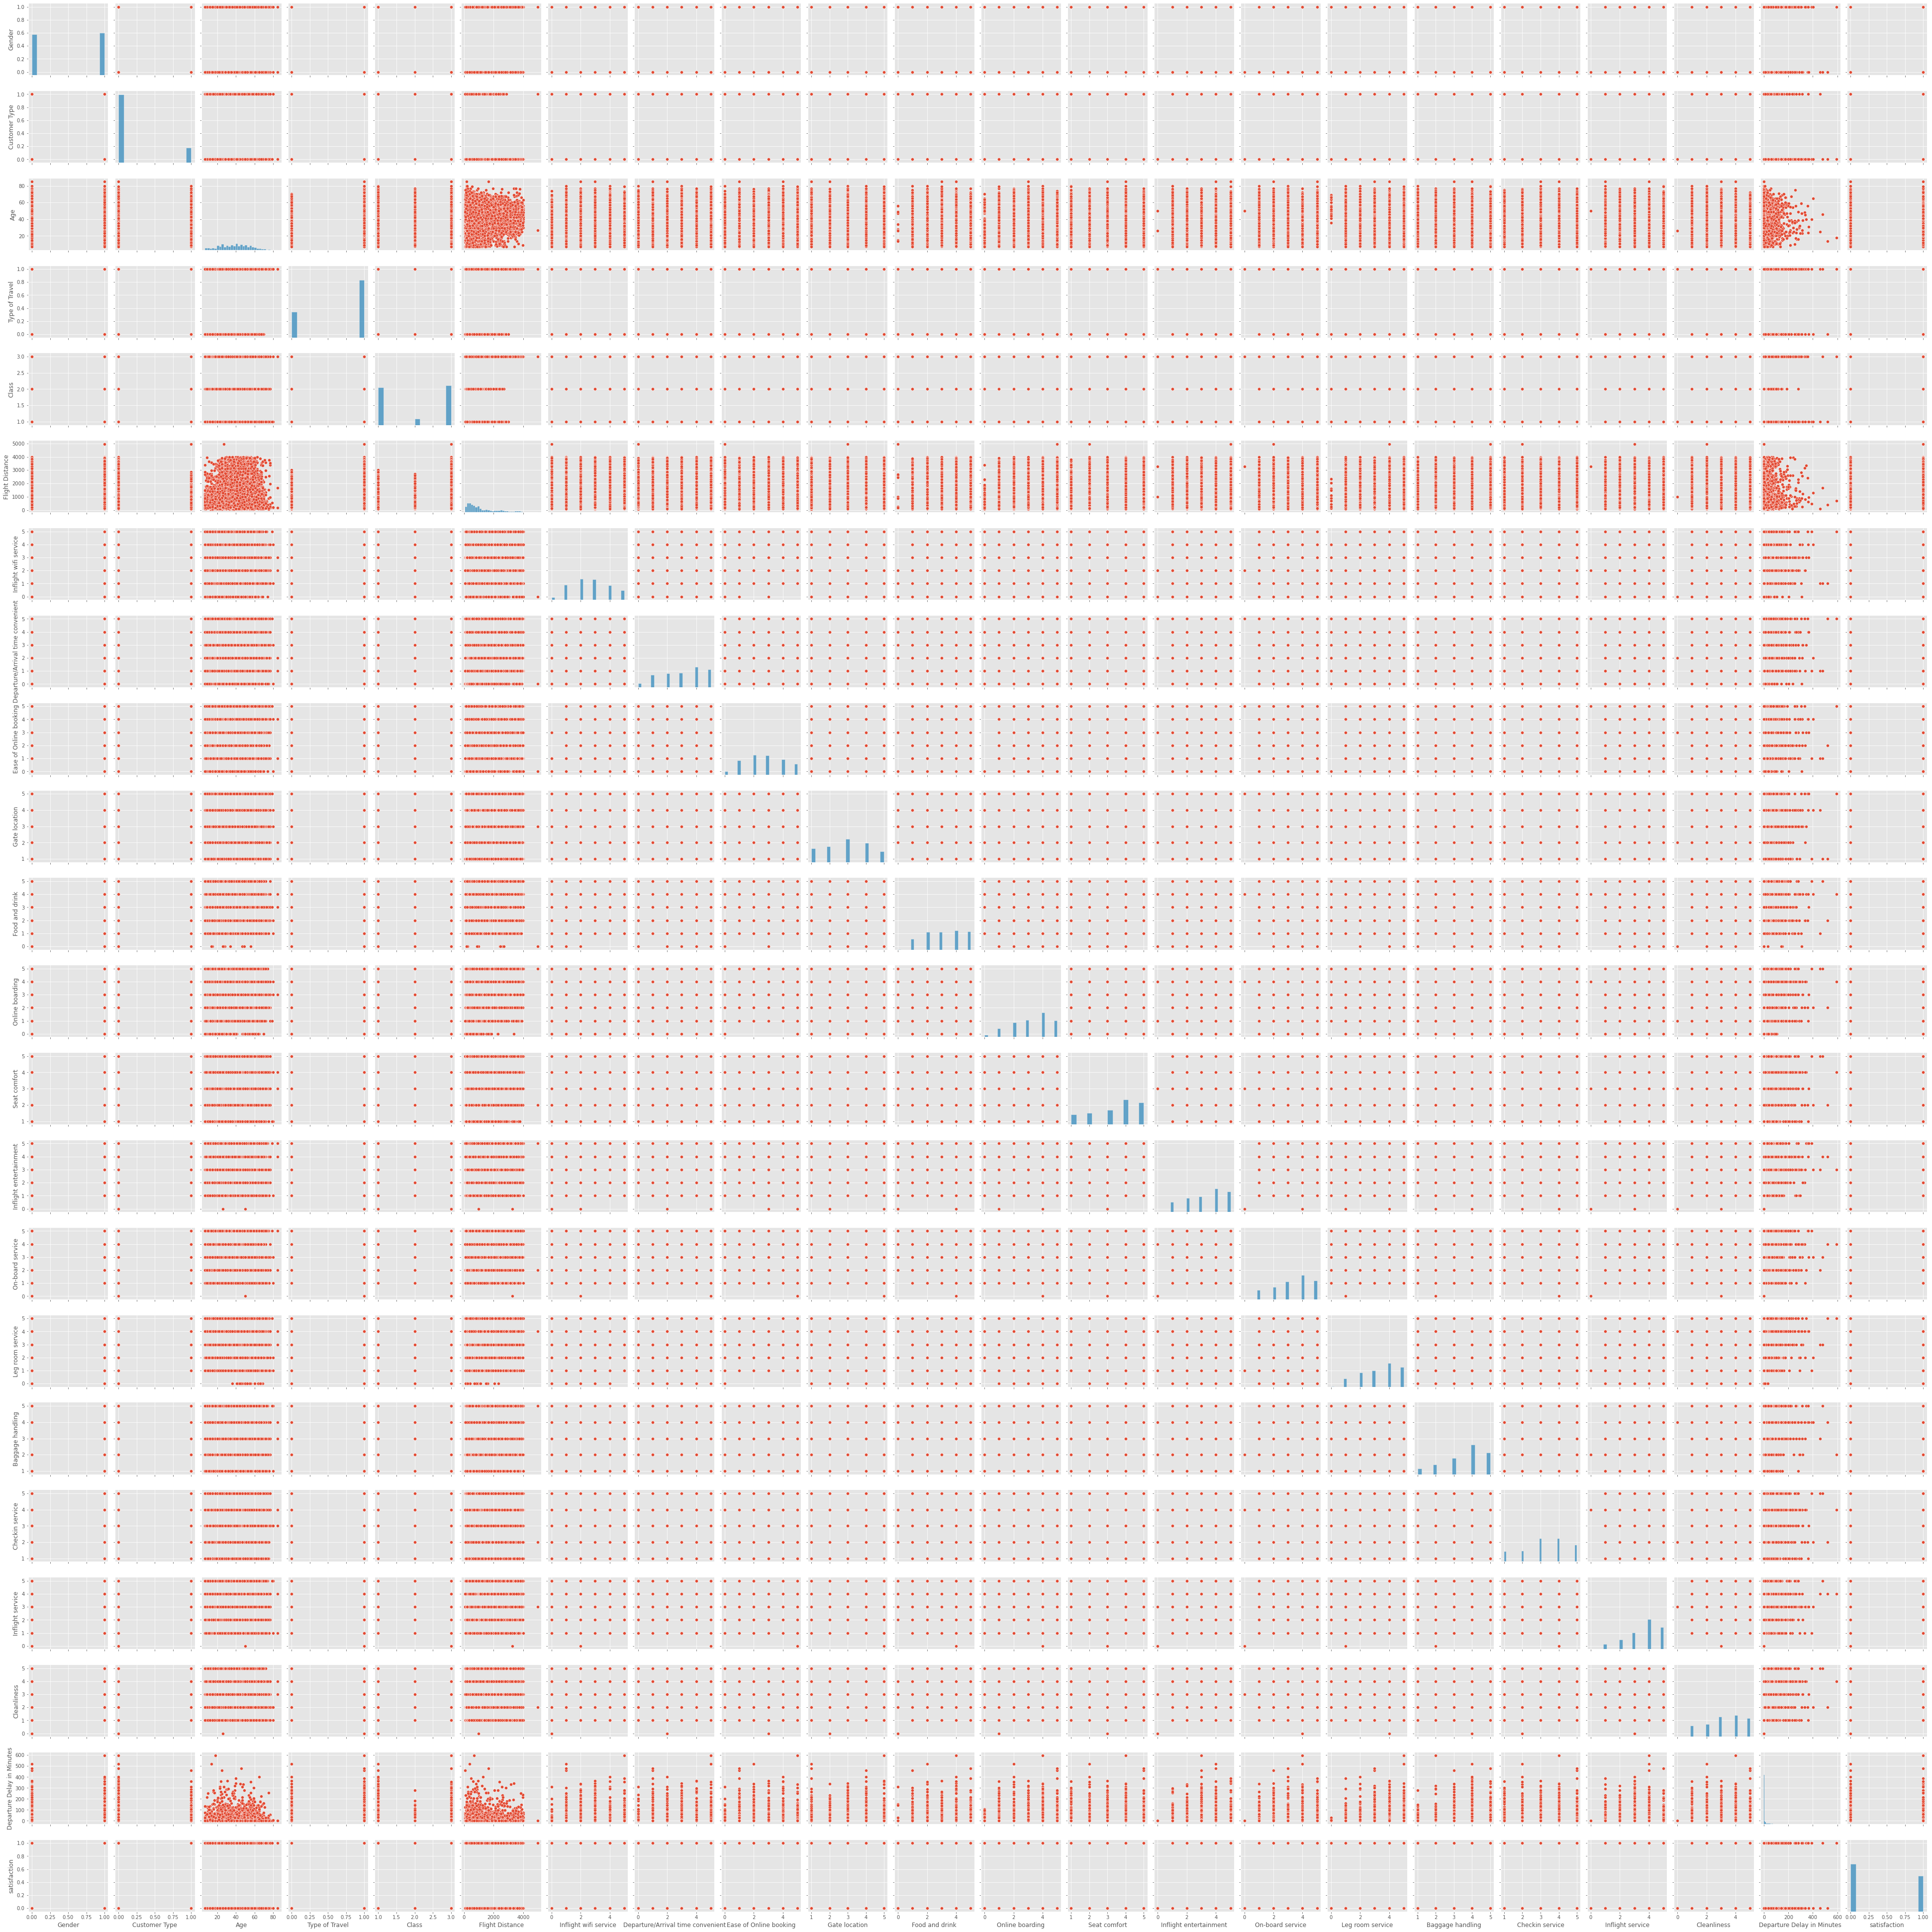
\includegraphics[width=0.9\textwidth]{pariplot_feature_data.png}
		\caption{Pairplot Feature Data US Airline Passenger Dataset}
        \label{fig:pairplot_feature}
  \end{figure}

